\documentclass[a4paper]{article}
\usepackage[utf8]{inputenc}

\usepackage[left=2cm,right=2cm,top=2cm,bottom=2cm]{geometry} % per definizione layout

\usepackage{titlesec}
\usepackage{graphicx}
%\usepackage{ifthen}

\usepackage{epsfig}

\usepackage{xcolor}
\usepackage{listings}

%\usepackage[a-1b]{pdfx}
\usepackage[pdfa]{hyperref}

\usepackage{url}
\usepackage{soul}

\usepackage{lscape}

% titoli grandi
\titleformat{\section}{\normalfont\LARGE\bfseries}{\thesection}{1em}{}

% titolo teorema
\newtheorem{definition}{Definition}

\title{\huge\textbf{Cyber Security Risk Assessment\\A.Y. 2020-2021}\\\medskip\Large\textbf{Final Report - Group 8\\Introduction to Smart Working in a Court}}
\author{Claudio Facchinetti \texttt{<claudio.facchinetti@studenti.unitn.it>}\\
Matteo Franzil \texttt{<matteo.franzil@studenti.unitn.it>}}

\begin{document}

\maketitle

\tableofcontents

\newpage

\begingroup
  
\section{Executive summary}
\label{sec:executive-summary}

This report is produced for the \textbf{Tribunal of Bengodi}.

While performing the assessment we found out several network configuration errors and some software vulnerabilities that could allow a malicious entity to access, modify and even destroy some of the core processes of the Tribunal. Nonetheless some of the problems we found could lead to restricted form of identity theft: a malicious entity could find the VPN access credentials of some of the users and operate unauthorized / illegal actions as if it is the user having legitimate access to the system.

More precisely the network configuration issues and the software vulnerabilities, some with a Base CVSS score of 10, could lead to, in the worst case scenario, millions of euros to be payed as fees and / or damage compensation.

The countermeasures we proposed at network level are based on basic security and networking practices we mainly learned during other courses in the University; we also proposed other countermeasures that are not related to the context of IT security that are, in our opinion, necessary.

For each of the countermeasures we proposed we also gave a cost estimate, which is based on the market offerings found over the Internet and also a new quantitative assessment to make sure that the cost were justified by its benefit.

The observation time was fixed at one year which looked reasonable as this proposal aimed to allow clerks to get their job done from home due to COVID-19; taking into account the vaccination campaign in Italy we don't expect the critical situation to last more than this time interval.

\bigskip
\hspace{10pt}

\bigskip
\hspace{10pt}

Work submitted in partial fulfillment for the course of \textit{Cyber Security Risk Assessment} - \textit{University of Trento} - \textit{a.a. 2020/2021}.
\medskip\\This work is original work, has been done by the undersigned students and has not been copied or otherwise derived from the work of others not explicitly cited and quoted. 
\medskip\\The undersigned students are aware that plagiarism is an academic offence whose consequence include failure of the exam.

\bigskip

\begin{tabular*}{\textwidth}{ c @{\extracolsep{\fill}} c }
	Claudio Facchinetti & Matteo Franzil\\
	223814 & 221214 \\
	\includegraphics[height=30pt]{drawable/firma-claudio.eps} & \includegraphics[height=30pt]{drawable/firma-matteo.eps} \\
\end{tabular*}
	
\clearpage
\section{Target of evaluation}
\label{sec:target-evaluation}

For the purposes of this report, the Tribunal of Bengodi provided us with a network scan of their premises. We used the available data to draw a preliminary mapping of their network in order to ease later work

Figure \ref{fig:initial-network} shows the state of the network. Since the scan was partially complete, we had to make several assumptions and edit the diagram slightly.

Floors are represented by the dotted circles. The leftmost one is the $1^{st}$ floor, the topmost one is the $2^{nd}$, the rightmost one is the $3^{rd}$, while the remaining small one is the ground floor. Thick black lines represent trunk connections between the default gateway and floor switches. We decided to address the lack of gateway IPs in some VLANs by adding a fictional firewall/router, whose networks are connected with light grey lines. Finally, this router is connected to the Prosecutor Investigator Labs and marked as \textit{Scanner Location}.

The rest of the diagram is fairly straightforward and uses VLAN tags along with color markings for better understandings of VLAN locations. The VPN access is located in the bottom right, connected to the Civil Court Clerks subnet (VLAN \verb=17=).

This approach, if left untouched, presents multiple flaws. Firstly, as it stands it's unclear whether traffic going to and from the VPN concentrator will be firewalled or will take a different route. This must be addressed first. Secondly, the VLAN \verb=17= is shared with the Prosecutor Head and Assistant subnet. Since we don't know if the two VLAN can contact each other (i.e. if there's a router segmenting them or not, which is hard to know with a simple scan), we need to make sure to segment the two into separate VLANs. This approach must be taken for all conflicting subnets (i.e. VLANs \verb=18, 40, 53=).

As it stands, deploying a VPN on such an architecture would be detrimental to security. In Section \ref{sec:summary-findings}), we propose some mitigations to this deployment.

\begin{figure}[!h]
	\centering
	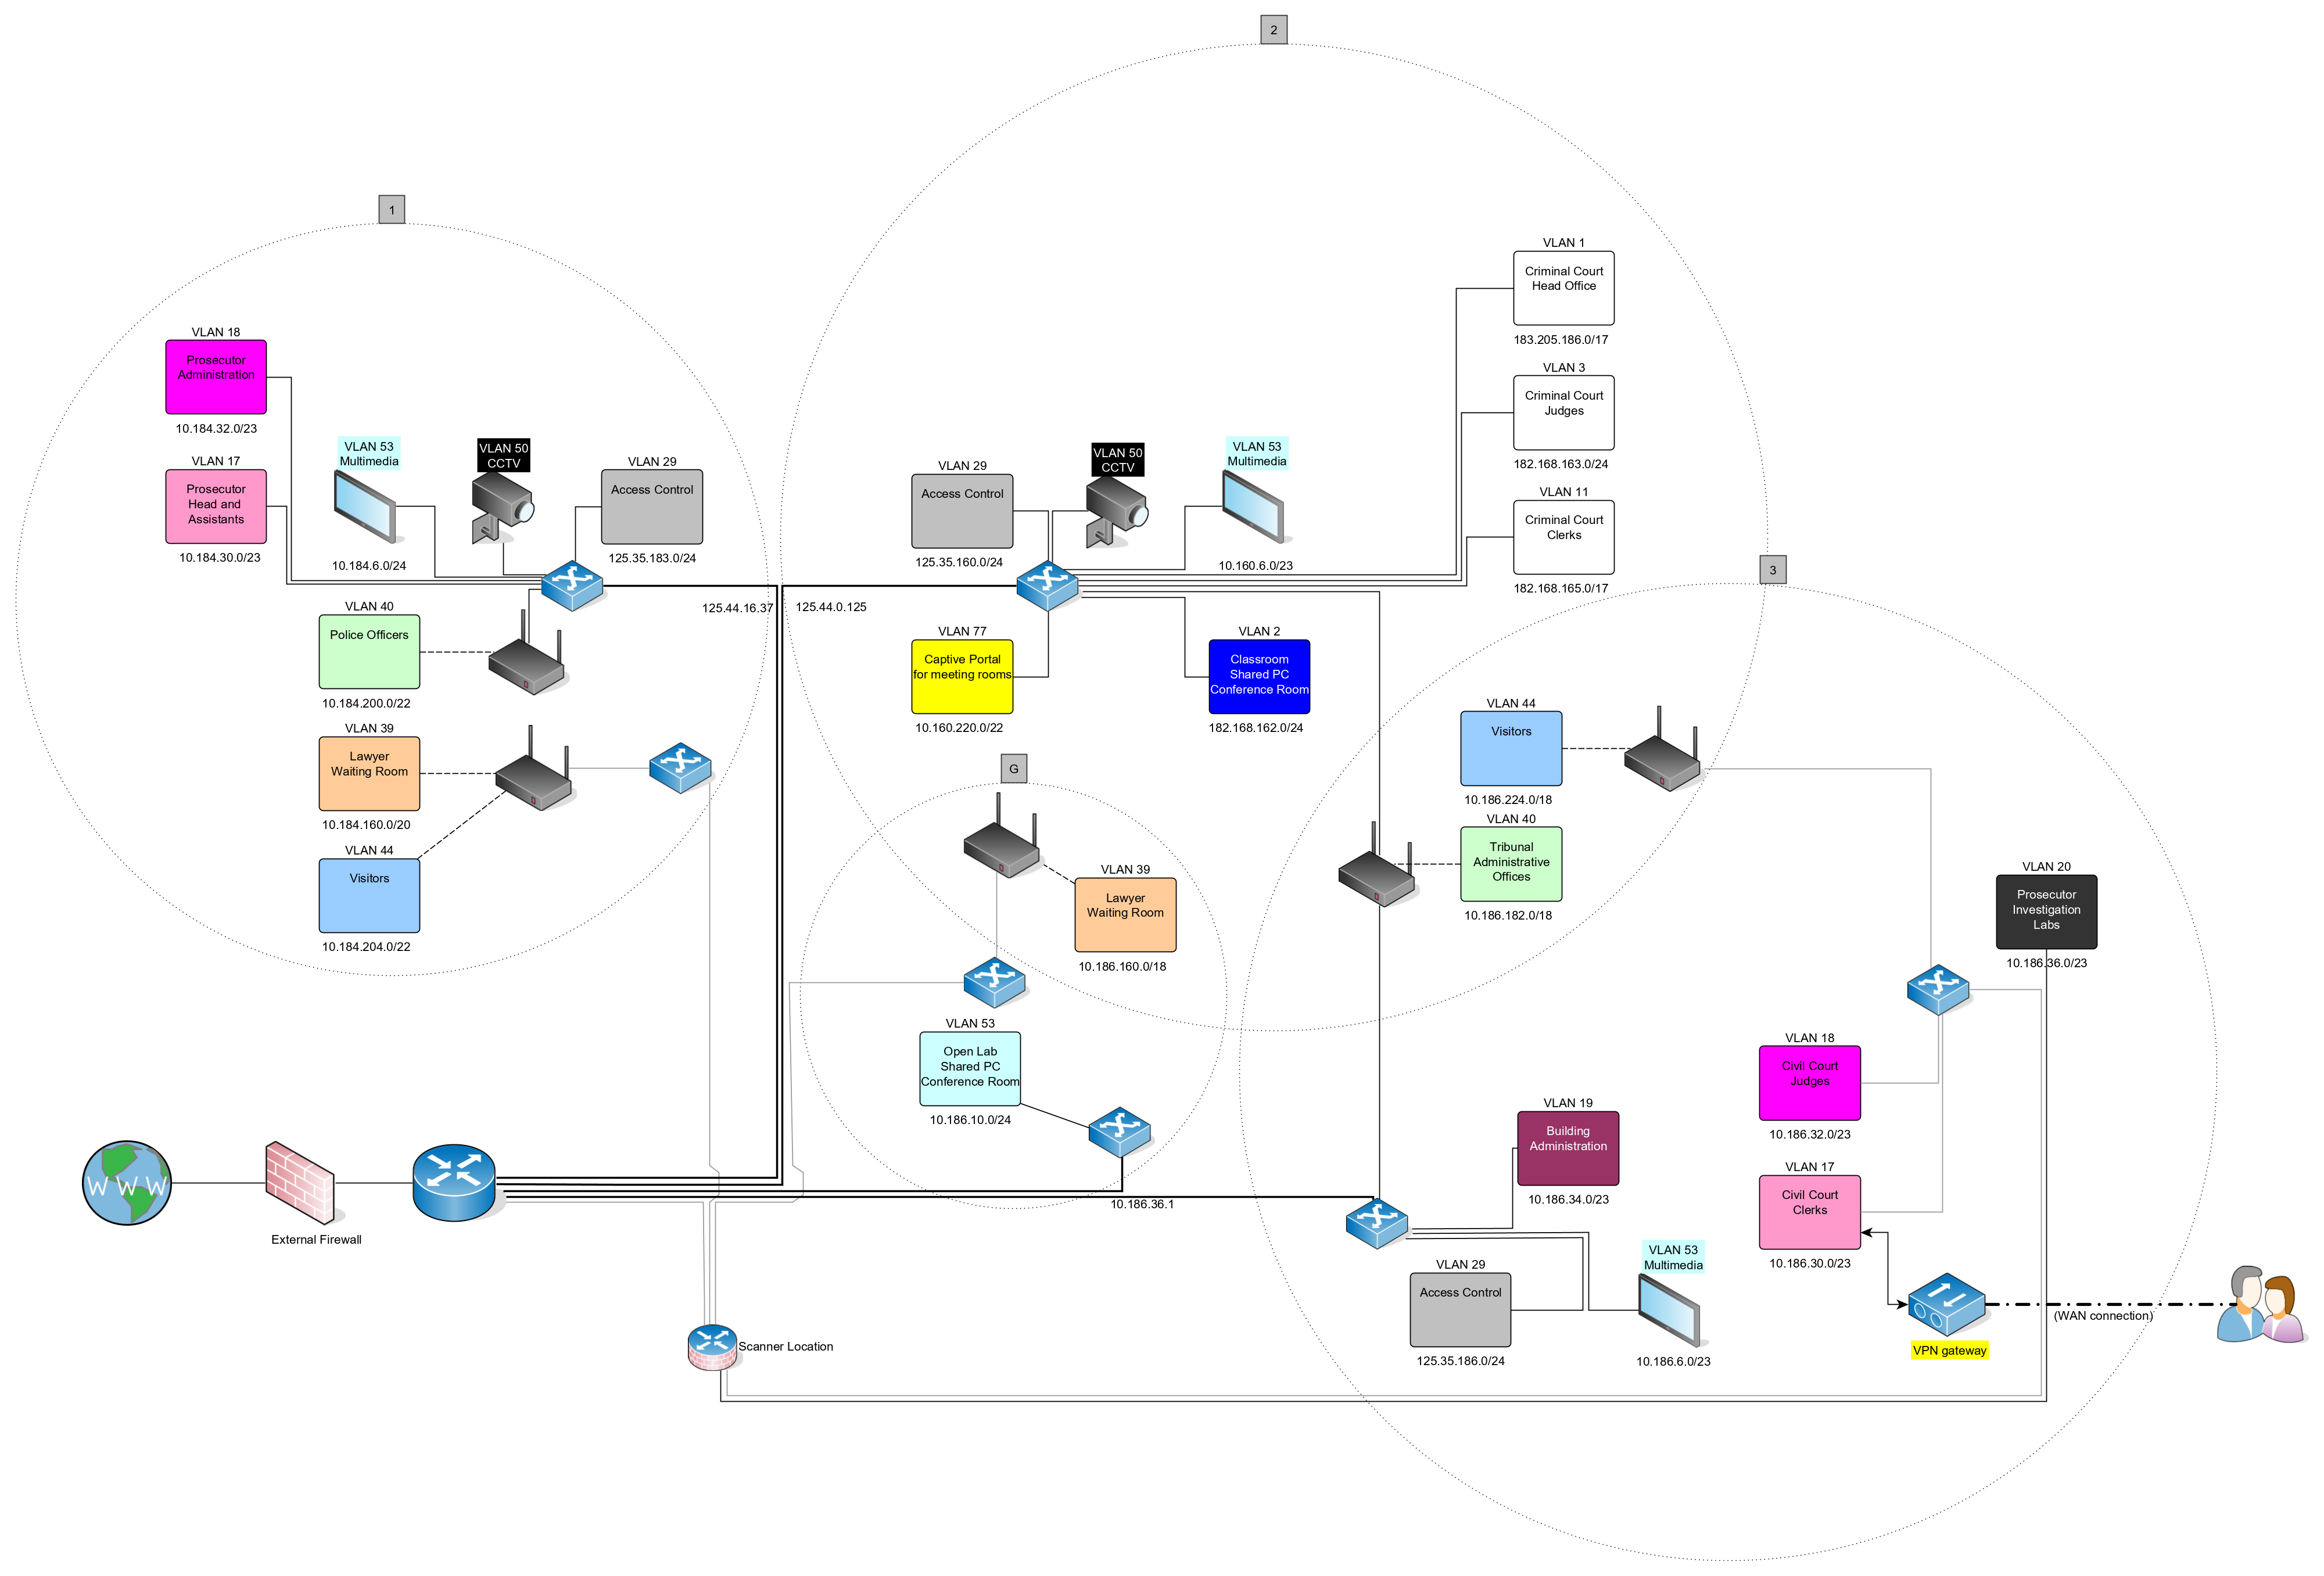
\includegraphics[width=\textwidth]{drawable/rete.png}
	\caption{Network diagram based on the Tribunal's provided scan.}
	\label{fig:initial-network}
\end{figure}

\clearpage
\section{Summary of findings}
\label{sec:summary-findings}

This section discusses the security problems identified for this scenario and our proposed mitigations.

\subsection{Architectural changes}

Figure \ref{fig:updated-network} shows our proposal in updating the network architecture in order to better suit modern standards and also to increase resiliency to attacks. These measures are the first and foremost that should be undertaken, and must go hand in hand with the countermeasures proposed in our qualitative and quantitative analysis in the next sections.

\begin{figure}[!h]
	\centering
	%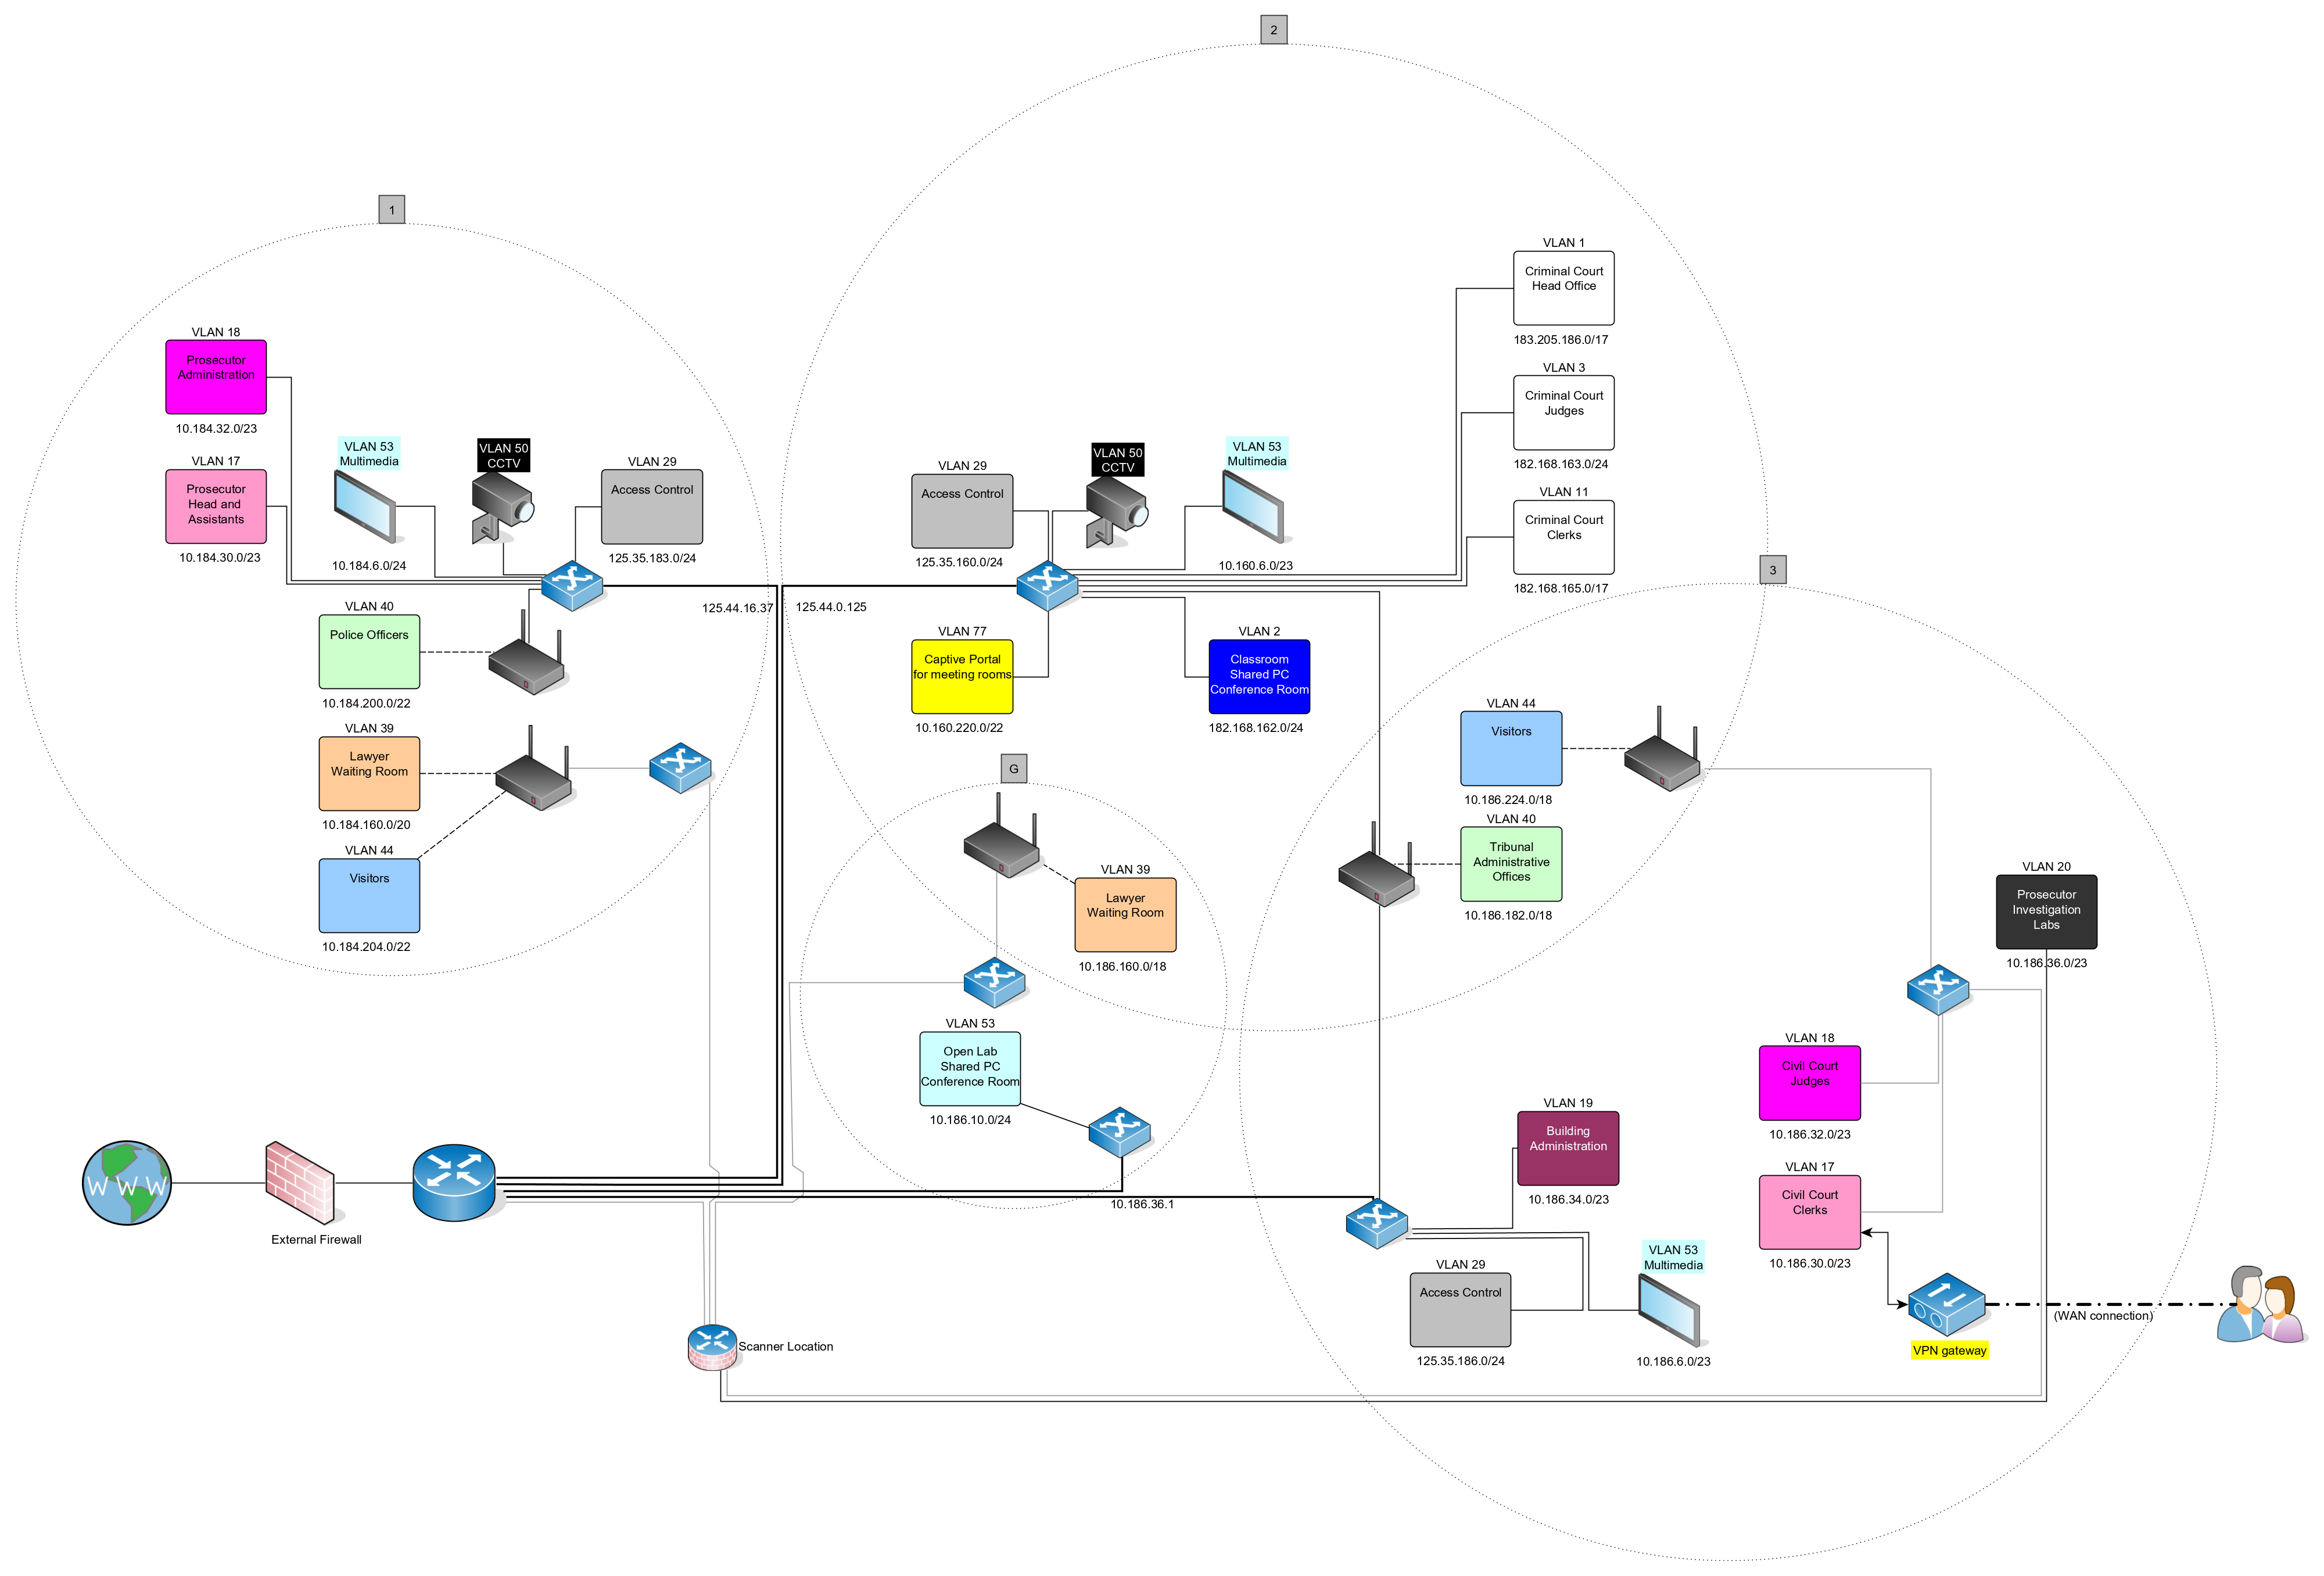
\includegraphics[width=1.4\textwidth]{drawable/rete.png}
	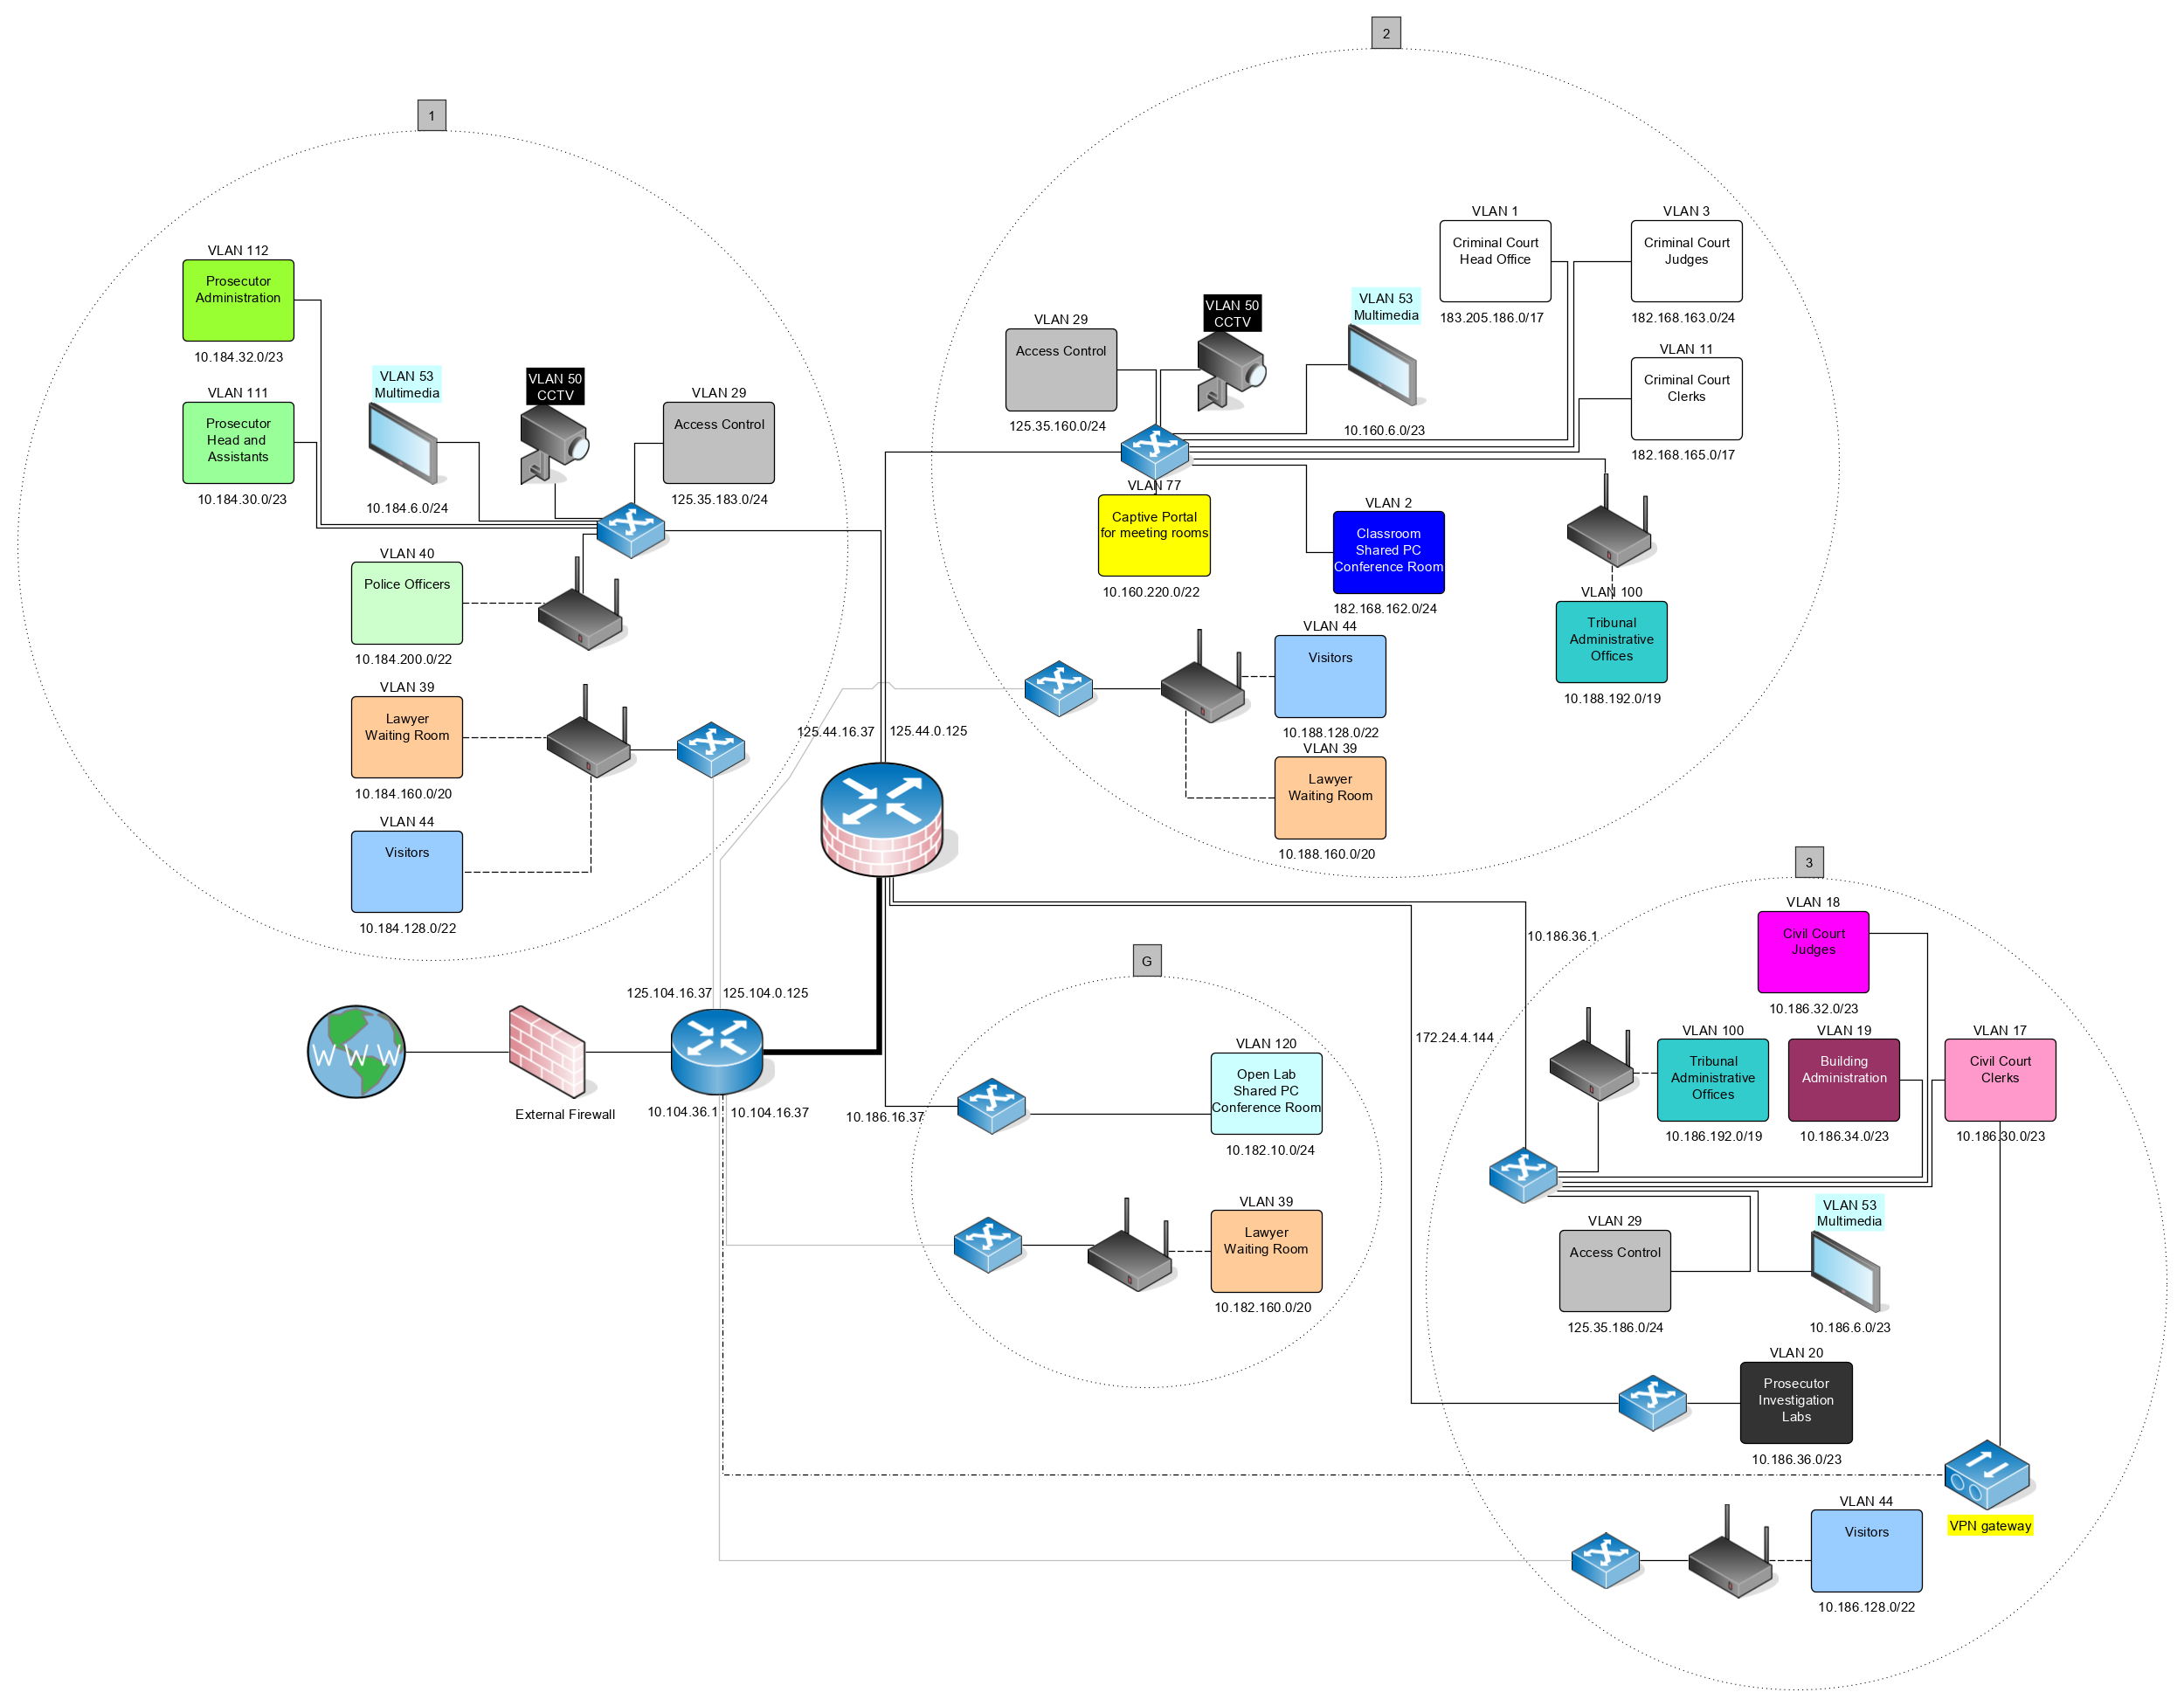
\includegraphics[width=\textwidth]{drawable/rete-updated.png}
	\caption{Architectural Description of the target and the proposed security mitigations to be deployed.}
	\label{fig:updated-network}
\end{figure}

First, we decided to re-number some VLANs as we realized some of them covered completely different sections of the Tribunal. Indeed, VLAN IDs \verb=17= and \verb=18= were shared between the Prosecutors and the Civil Court, and the former were renamed to \verb=111= and \verb=112=. While we do know that inter-VLAN routing should be disabled, we cannot make sure that really there is no route between them, and we want to enforce a "VLAN/IP" policy so that no two subnets share an IP or a VLAN ID. In this case, it was extremely important to segregate them as VLAN \verb=111= was found to be ridden with vulnerabilities in the provided scan.

The same approach was taken for the for the Shared PC Conference Room at ground floor, moved to VLAN \verb=120=, and the Tribunal Administrative Offices, moved to VLAN \verb=100= away from the Police Officers one. We undertook several redesigns of the cable layout, and our best suggestion is to reconfigure the network in order to either use the only firewall as both a gateway firewall and inter-network firewall, or to buy a new apparatus and deploy it such that the communication between any two VLANs is secured. These costs are later discussed in the quantitative analysis. 

We also took steps in order to make sure that subnets related to visitors are not only logically but also physically separated from the rest of the network. Indeed, the scan showed such subnets without a gateway, and we addressed it by creating new fictitious IPs for a gateway located before the central firewall but after the gateway firewall.

\begin{figure}[!h]
	\centering
	%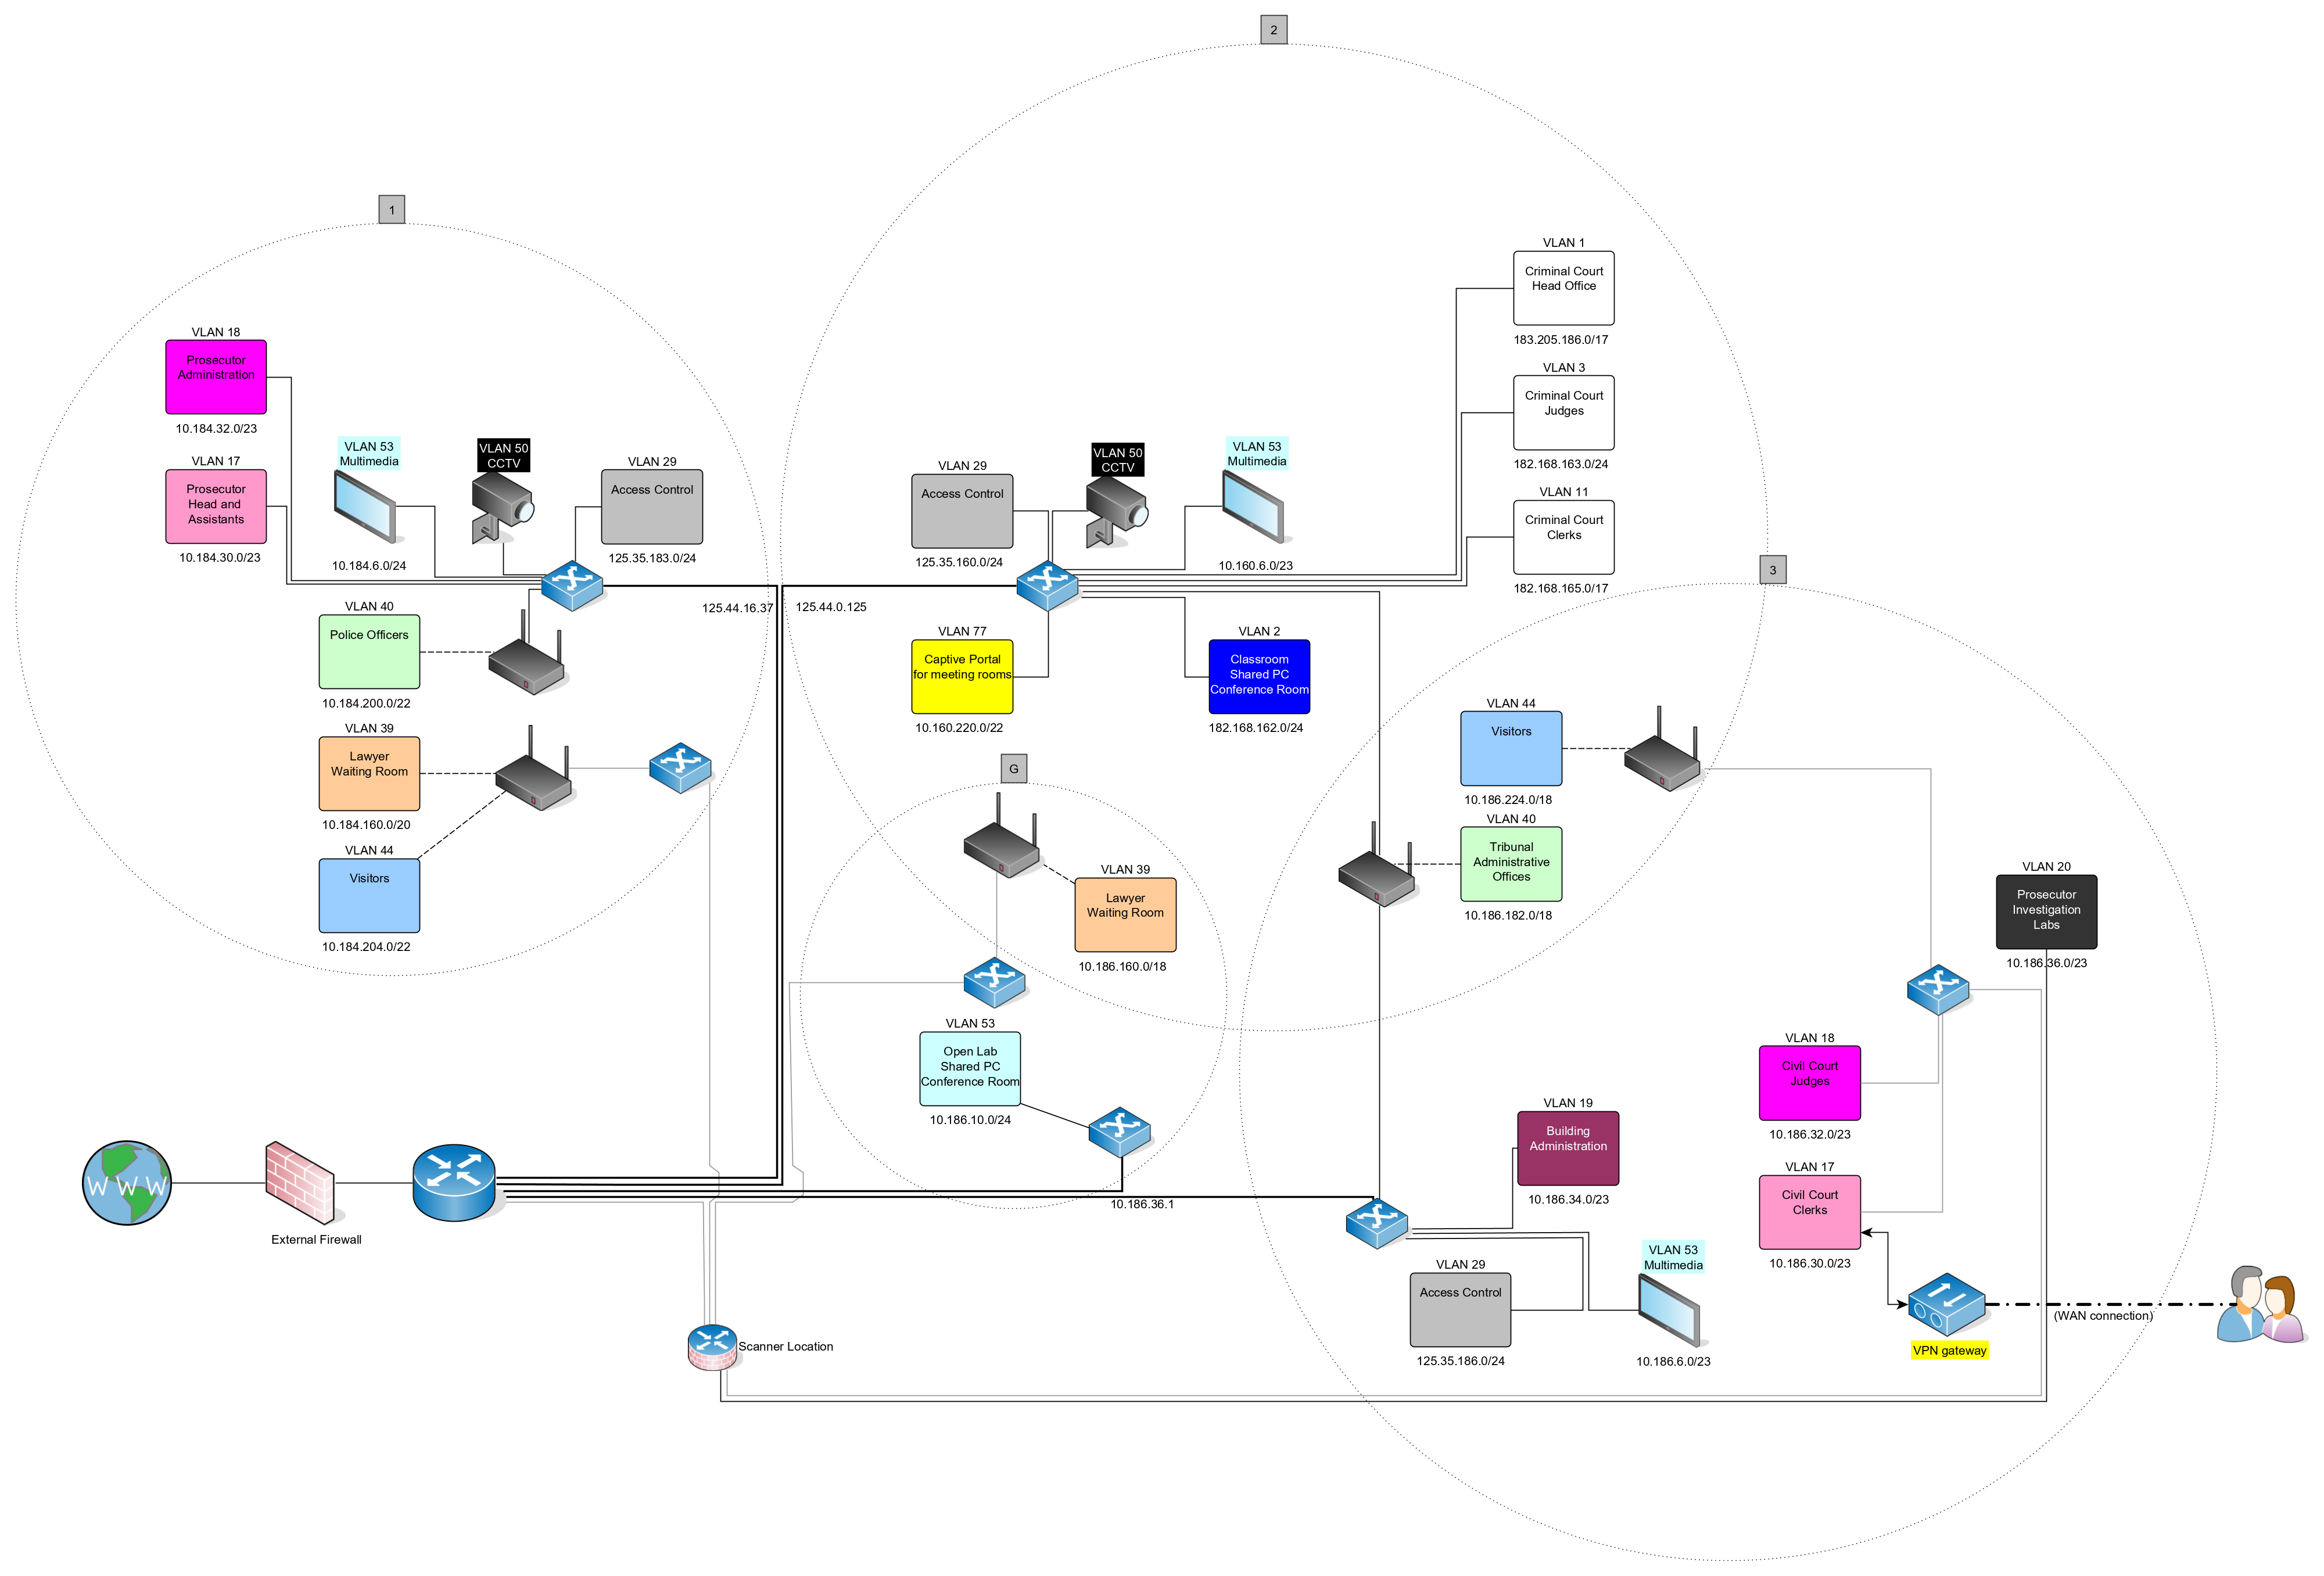
\includegraphics[width=1.4\textwidth]{drawable/rete.png}
	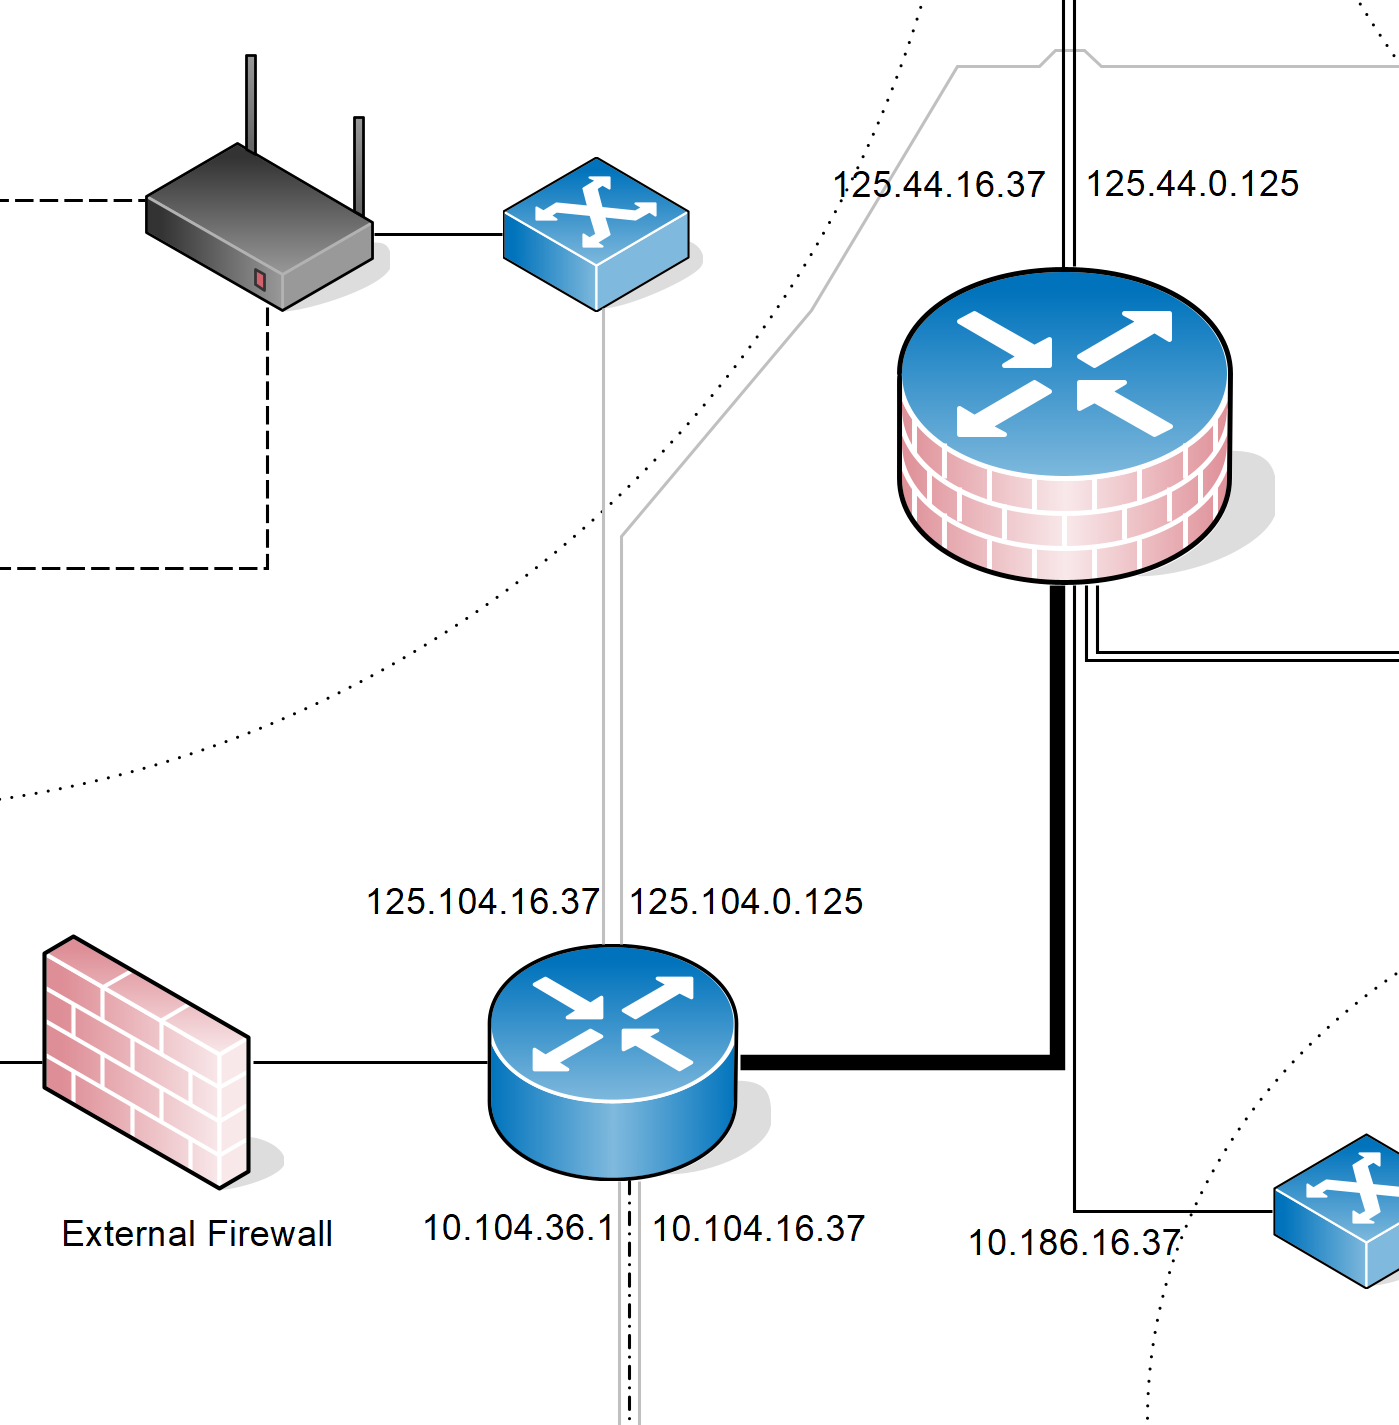
\includegraphics[width=0.5\textwidth]{drawable/detail-network.png}
	\caption{Enlarged snippet of the network diagram. We can see the external firewall, the initial gateway, and the inter-network firewall.}
	\label{fig:detail-network}
\end{figure}

Finally, in the diagram we moved some subnets around and introduced some logic in the IPs. Now, in most subnet IPs, the second group now reflects the floor of the subnet and VLAN itself. This caused the split of two subnets, mainly those related to visitors and hotspot access points. For example, subnet \url{10.186.224.0/19} was split into \url{10.188.128.0/22} and \url{10.186.128.0/22} for the Visitors subnet, with \verb=188= denoting the second floor and \verb=186= denoting the third. In general, this was done in order to avoid some overlapping that were present in the provided list. In the wake of this final suggestion, we also want to promote a full revision of all IPs (as this diagram is only meant to be a guideline) and firewall rules.

\subsection{Main analysis}

After completing our architectural redesign, we focused on the qualitative analysis. Our findings showed that while most supporting assets did have their fair share of High risk, the most at-risk ones were the VPN and log server(s) and the networking devices. This goes to show how fundamental it is and it would become the network architecture if one were to implement the suggested VPN system.

We took prompt action in order to secure and mitigate risk as much as possible. Our main suggested controls include the deployment of guards in the data center, redundancy, automated fail-over detection, and in general methods that allow enforcement of business continuity. We also stressed the need of installing a new inter-network firewall and enforcing employee policy in order to prevent undesirable social engineering attack vectors.

In the end, while the residual risk was almost flattened for some assets such as the VPN server itself, most primary assets did end up with a medium residual risk. However, we believe that it is an acceptable level of risk when taken into account jointly with the proposed quantitative countermeasures.

Indeed, our quantitative analysis focused on the possible monetary impact of several cyber attack scenarios on what we thought we were the most compromised machines in the system. Firstly, we collected the most prominent CVSS vulnerabilities from the provided Nessus scan. Secondly, we identified key systems and assigned IDs to them, enumerating their importance and their CVSS scores. For each of them, we discussed their importance and the probability of it being used as an attack vector for a cyber attack.

We then condensed the obtained data into a table in step 3, contextualizing attacks into five different possible main targets: the external firewall, the judicial software server, the VPN server, the log server, and a Clerk's PC. For each of them, we calculated the impact and the likelihood of an attack, first in a day, then amortized on a year.

Finally, we collected information about our controls implemented in the qualitative report, and researched their cost. After obtaining a reasonable estimate, we used that information to re-do the impact and likelihood calculation with the countermeasures.

What we found out was that due to mainly the GDPR-complying fines, the worst possible scenario would be an attack on the VPN server, with its estimated cost ranging in the tens of millions of euros. Additionally, other sensitive equipment such as the Clerks' PCs and the judicial software server were deemed risky of multi-million incidents. While the countermeasures did sharply decrease such a risk, the residual risk still remains in the same order of magnitude, and is almost impossible to completely mitigate, given the circumstances and the importance of the data managed by the tribunal.

\clearpage
\section{Risk analysis}
\label{sec:risk-analysis}

\subsection{Preliminary Qualitative Analysis}

The complete summary of results can be found in the document  \url{SecRAM-worksheet.xlsx} submitted as integral part of the current report.

As a first step we identified the primary assets and also assessed their impact as can be seen in parts 1.1 and 1.2 of the \url{SecRAM-worksheet.xlsx} document. 

Out of all the primary assets we identified the most critical one for the application of the smart working procedure in the court are:

\begin{itemize}
    \item the VPN service and associated credentials;
    \item the certified email service (\textit{PEC}) and associated credentials.
\end{itemize}

At step 1.3 of the attached document document we identified the supporting assets linked to every primary asset, but in particular we found the following ones related to the previous supporting assets:

\begin{itemize}
    \item personnel's PCs;
    \item VPN server(s);
    \item personnel;
    \item server room(s);
    \item network devices.
\end{itemize}

After identifying these ones we proceeded identifying, in step 2.1, possible threats for every supporting asset; out of all the possible vulnerabilities the most important ones are:

\begin{itemize}
    \item partial or total destruction, for all of the supporting assets listed before;
    \item compromise of information, for all of the supporting assets listed before;
    \item theft, for all of the supporting assets listed before except for the server room (s).
\end{itemize}

For each vulnerability we also identified related threats and we will report here the most relevant one.

For the compromise of information we identified:

\begin{itemize}
    \item non-adherence to security practices;
    \item firmware or software vulnerability.
\end{itemize}

For partial or total destruction we identified that the threats can come in different forms depending on the asset, but they can all be classified into the following groups:

\begin{itemize}
    \item accidental damage, either man-made or not;
    \item sabotage;
    \item natural disaster.
\end{itemize}

The threats reported above are also those with the highest risk level, as can be seen in the step 3.2 of the attached document.

After this step, we concluded that while most supporting assets did have a high level of risk, some vulnerabilities in them (some in the personnel PCs, but also in the judicial software server and the power supply) were presenting a risk level low enough to justify not adding controls to them.

In step 4, for the rest of the vulnerabilities, we identified some controls that can be put into place in order to reduce the risk level of the all the threats identified; in particular the most immediate controls we proposed can be split into the following categories:

\begin{itemize}
    \item physical restrictions, such as guards locked doors;
    \item networking structure enhancement, such as better isolation of VLANs and better disposition of the VPN server;
    \item keeping software up to date.
\end{itemize}

In step 5 we identified the residual risk level for each primary asset which is \textit{"Medium"} for every single primary asset, having a scale of three risk levels: \textit{"High"}, \textit{"Medium"}, \textit{"Low"}.

\subsection{Quantitative Analysis}

The complete summary of results can be found in the document \url{CVSS-worksheet.xlsx} submitted as integral part of the current report.\footnote{Note: the CVSS-worksheet file steps refers to all systems and CIDR based on their new mappings, as anticipated in section 2. This is in order to avoid confusions. A separate tab, \url{Annex-VLANList}, is provided in the Excel file in order to have a lookup table for old VLAN IDs/CIDRs.}

At Step 1 we identified the vulnerabilities present in the network before the risk analysis and have identified the key systems. They are summarized in \url{CVSS-worksheet.xlsx}, tab \url{Step1}.

First, we derived the most important systems for each VLAN. Then, for each system, we assigned a unique ID and identified key vulnerabilities. The CVSS column refers to the highest identified vulnerability on that system, as a row may contain two or more vulnerabilities. Furthermore, we chose to operate only on vulnerabilities rated CVSS 4 or higher, in order to better focus on the key issues that have to be addressed promptly. Among the systems we analyzed, we believe the most important are 11B and 111F (the judicial process servers), although there exist some PCs with CVSS vulnerabilities rated 10 (mainly, those featuring EOL operating systems). Throughout the system, finally, other key vulnerabilities usually fall down on expired TLS certificates and insecure ciphers.

At Step 2 we have identified the power of attackers that are consistent with our key stakeholder (see section 1). In our scenario, our priority is to secure all endpoints of the judicial process server from external network attacks. We believe that, in 2020, social engineering is fundamental but more often than not the first door hackers want to open is the remote one\cite{ferrarella_2018}\cite{salerno_2018}. Therefore, in our scenario, we decided to prioritize most remote attacks. This translates in focusing on remote vulnerabilities to the judicial process server (systems \url{111C}, \url{111D}, \url{111E}, \url{111F}). In order to get an acceptable security level, all PCs in the system must also be updated to the latest OS level patches (systems \url{19C}, \url{1A} in particular). However, given the state of the network, our recommendation is to also carry over as many mitigations possible, by checking the results of the next step.

While online attacks may be imminent, particular attention still must be given to potential mole or infiltration attacks\cite{online_2011}. In fact, in our step 3.1 we calculated the overall impact and likelihood for selected cyber attacks scenarios, and potential vectors deriving by both fully remote attacks or locally assisted attacks. Data is reported in Table \ref{tab:step3} for the key assets. Full details are available in \url{CVSS-worksheet.xlsx}. 

\begin{center}
    \label{tab:step3}
    \begin{tabular}{|l|l|l|l|}
    \hline
    Component & Impact & Likelihood & Risk (1 year)
    \\
    \hline
    External firewall     & € 8000      & \verb=0.14= & € 2.174.82    
    \\
    \hline
    Judicial Software Server     & € 10018000       & \verb=0.40=       &  € 70.529.267,78 
    \\
    \hline
    VPN Server     &  € 11.950.750,00        & \verb=0.51=       &  € 80.043.484,77 
    \\
    \hline
    Log server     &  € 12.400,00        & \verb=0.10=       &  € 1.064,62       \\
    \hline
    Clerk's PC     &  € 9.300,00        & \verb=0.40=       &  € 1.557.012,34 
    \\
    \hline
    \end{tabular}
\end{center}

Finally, at step 4 we identified the total costs of our proposed countermeasures (for € 176.400,00 in total). We used several sources to compile this information\cite{avfirewalls}\cite{basics_2020}\cite{limited}. Additionally, we measured the residual likelihood and therefore the residual risk after we have applied the countermeasure. This was done using the amortized costs for one year. They are finally listed in Table \ref{tab:step4} with the related costs side.

\begin{center}
    \label{tab:step4}
    \begin{tabular}{|l|l|l|l|}
    \hline
    Component & Residual Likelihood & Residual Risk \\
    \hline
    External firewall     & \verb=0.14=       &  € 915,71        \\
    \hline
    Judicial software server     & \verb=0.40=       &  € 20.642.712,52
    \\
    \hline
    VPN Server     & \verb=0.51=       & € 17.152.175,31
    \\
    \hline
    Log server     & \verb=0.10=       & € 266,16
    \\
    \hline
    Clerk's PC     & \verb=0.40=       & € 79.846,79
    \\
    \hline
    \end{tabular}
\end{center}

\clearpage

\section{Annex}
\label{sec:annex}

As an integral part of the report, we attach the following documents:

\begin{itemize}
    \item Excel document reporting the application of SESAR SecRAM method (see file \url{SecRAM-worksheet.xlsx}).
    \item Excel document reporting the application of CVSS Quantitative method (see file \url{CVSS-worksheet.xlsx}).
\end{itemize}

\clearpage

\endgroup

\addcontentsline{toc}{section}{References}

\bibliographystyle{IEEEtran-sorted-tt}
\bibliography{biblio}

\end{document}
